Based on the machine learning and deep learning applications for the task of breast cancer detection established in Chapter~\ref{ch:chapter-litsurvey}, and the datasets available for this project, design decisions specific to the deep learning pipeline implemention will be covered, along with the reasoning behind the choice of datasets to use and general considerations.

\section{Datasets Decision}

An early design decision taken as a group consisted of electing which datasets to use, as Chapter~\ref{ch:chapter-ethics-datasets} revealed that each dataset has different characteristics. Despite being widely used in existing literature (see Chapter~\ref{ch:chapter-litsurvey}), popular feature-based datasets containing extracted mammogram data such as the WBCD dataset \citep{Wolberg1995} will not be used, as the objective of using deep learning models such as CNNs is to learn which features to extract by using the raw image in 2D space rather than data flattened into 1D arrays. If extracted features such as the ones from WBCD were used, then already successful machine learning algorithms such as SVMs or DTs could be used instead of deep learning techniques.\\

From a clinical point of view, the mini-MIAS dataset is interesting as it contains both abnormal cases and normal cases, resulting in three classes (normal, benign and malignant cases). Its smaller size makes it useful for initial prototyping but has the downside of requiring more image processing techniques such as data augmentation to generate enough data to feed into the deep learning model. The different types of breast backgrounds (see Section~\ref{sec:ethics-mini-MIAS-dataset-description}) is not considered during training to avoid further splitting the dataset.\\

The CBIS-DDSM dataset was chosen over the DDSM dataset as it is an updated version of the older DDSM dataset, and is curated by a trained mammographer. Additionally, it uses uncompressed images in DICOM format rather than LJPEG format, which is a deprecated format nowadays, resulting in much higher quality imagery.  Indeed, the large uncompressed format offered by DICOM means that the mammograms can be fed into the CNN with larger sizes, allowing the model to potentially learn more low-level features. Another plus is that the dataset is already split into training/testing sets, allowing for accurate performance comparisons with other papers using the same dataset. Despite the CBIS-DDSM dataset containing two different views (CC and MLO), the mammograms in each case are treated as separate individual images due to the limited number of samples available.\\

%%%%%%%%%%%%%%%%%%%%%%%%%%%%%%%%%%%%%%%%%%%%%%%%%%%%%%%%%%%%%%%%%%%%
%%%%%%%%%%%%%%%%%%%%%%%%%%%%%%%%%%%%%%%%%%%%%%%%%%%%%%%%%%%%%%%%%%%%
%%%%%%%%%%%%%%%%%%%%%%%%%%%%%%%%%%%%%%%%%%%%%%%%%%%%%%%%%%%%%%%%%%%%

\section{Deep Learning Pipeline Design Analysis}

The deep learning pipeline implemented for the task of breast cancer detection can be broken down in four distinct phases, which are condensed in Figure~\ref{fig:design-flowchart}:

\begin{itemize}
    \item \textbf{Data pre-processing}: loading a dataset in memory and processing it to gather image-label pairs for the classification task.
    \item \textbf{Model training}: creating a CNN model that can fit the data to learn the training set samples. Predictions are carried out once the model finishes training on the validation and test sets.
    \item \textbf{Result visualisation}: the model's performance is evaluated by calculating various metrics and plotting predictions.
    \item \textbf{Fine tuning}: a bag-of-tricks approach is used, experimenting various deep learning techniques.
\end{itemize}

\begin{figure}[ht]
\centerline{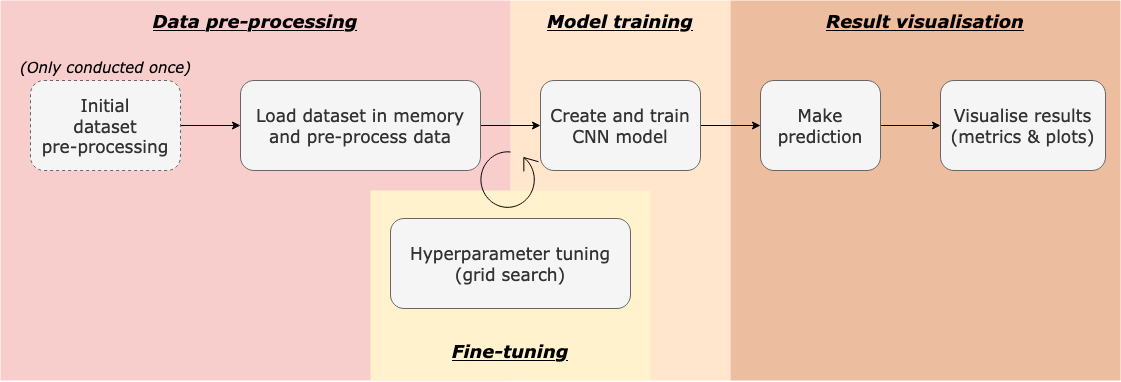
\includegraphics[width=\textwidth]{figures/design/design flowchart.png}}
\caption{\label{fig:design-flowchart}A high-level flowchart of the breast cancer detection deep learning pipeline to implement, separated into data pre-processing, model training, results visualisation and fine-tuning.}
\end{figure}

%%%%%%%%%%%%%%%%%%%%

\subsection{Data Pre-Processing}

\subsubsection{Dataset balance}
\label{sec:design-dataset-balance}

As this is a classification task, it is essential to visualise the distribution of classes in the datasets to determine whether the dataset balance is skewed or not (whether some classes are much more frequent than other classes \citep{Geron2019}). The class distributions are plotted in Figure~\ref{fig:design-datasets-balance}.

\begin{figure}[h]
\centering
\begin{subfigure}{.5\textwidth}
  \centering
  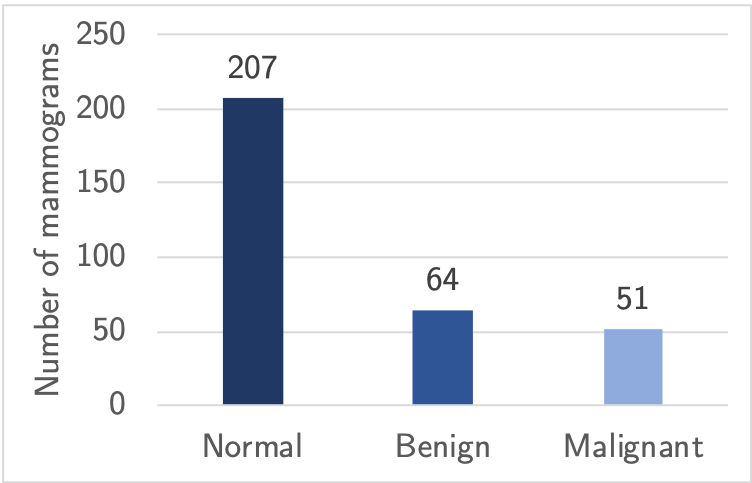
\includegraphics[width=0.94\textwidth]{figures/design/mini-mias-balance.png}
  \caption{mini-MIAS class distribution.}
  \label{fig:design-mini-mias-balance}
\end{subfigure}%
\begin{subfigure}{.5\textwidth}
  \centering
  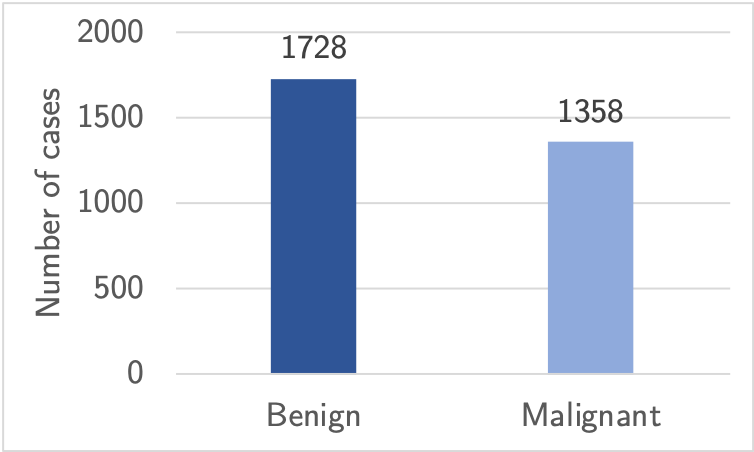
\includegraphics[width=\textwidth]{figures/design/cbis-ddsm-balance.png}
  \caption{CBIS-DDSM class distribution.}
  \label{fig:cbis-ddsm-balance}
\end{subfigure}
\caption{\label{fig:design-datasets-balance}Class distribution for the mini-MIAS and the CBIS-DDSM datasets.}
\end{figure}

These bar charts reveal that the mini-MIAS dataset is heavily imbalanced as the distribution is not uniform, which must be taken into account to avoid training a biased CNN model. Potential solutions to counter this imbalance would be to either:
\begin{itemize}
    \item \textit{undersample} the dataset by dropping images altogether;
    \item \textit{oversample} the dataset, which can be achieved via data augmentation,
    \item include \textit{class weights} to give more importance to under-represented classes. 
    %https://datascience.stackexchange.com/questions/13490/how-to-set-class-weights-for-imbalanced-classes-in-keras 
    %https://www.tensorflow.org/tutorials/structured_data/imbalanced_data#class_weights
\end{itemize}

Undersampling the dataset can be considered inefficient as it will diminish the number of samples the model could learn from by dropping samples from the majority class \citep{Liu2009}. As the datasets are already very small (maximum of 10,239 images in CBIS-DDSM), undersampling would be a poor strategy as it may discard useful features that could be learned. Consequently, oversampling by creating new artificial images resembling the original data is a viable solution as it was proven to increase accuracies (see Section~\ref{sec:litsurvey-data-augmentation}). Alternatively, a cheaper option in terms of computing power that does not require the dataset to be touched would be to add class weights, which will cause the loss to become a weighted average giving more importance to less frequent classes \citep{Zhu2018}.

\subsubsection{Dataset split}

The dataset is immediately split between a training set and a testing set to avoid any form of data snooping, which corresponds to the poor practice of making design decisions (either voluntary or involuntary) after having viewed the data and detecting patterns that could lead to favouring certain models or hyperparameters above others. Due to the small size of the datasets used and to avoid causing further imbalance to the datasets, the splits are not randomly sampled. Instead, stratified sampling is used, which consists of maintaining representative samples from the data in both the training and the testing sets to avoid introducing sampling bias.\\

An 80\%/20\% split, often used in machine learning and seen in breast cancer detection papers \citep{Yue2018}, is used to split the mini-MIAS dataset. The CBIS-DDSM does not need to be manually divided as it was already split with the appropriate stratification when it was designed \citep{Lee2017}. After this step, only the training set is utilised until the final results evaluations. The testing set is placed aside and forgotten about to avoid any form of cheating.\\

The assumption that the data never changes during the development of the project is made through fixed random number generator seeds (see Section~\ref{sec:implementation-results-reproducibility}). Not using a random generator with a fixed seed would cause different samples to be extracted into the training and testing sets every time the code is executed, thus neglecting the results. 

\subsubsection{Data loading}

The mini-MIAS dataset is very small in size (339 Mb before pre-processing, 202 Mb after pre-processing), containing only 322 images. It can therefore be loaded into memory without any data loading optimisation techniques. However, the CBIS-DDSM dataset is much larger, containing 10,239 images that cover 163.6 Gb of disk space. The dataset therefore cannot be loaded in memory in a single import and needs to be loaded in batches to be fed into the CNN sequentially. % mention batches and caching

\subsubsection{Data normalisation}

Images are resized to a target size during import to scale them down (CBIS-DDSM images are larger than 3000 x 5000 pixels)  and to avoid having inconsistent inputs. Observing the pixel intensities of the images found in the datasets reveal that they correspond to integers ranging from 0 to 255. However, because the weights in neural networks are small, having such large input values can disrupt and slow down the training process, ultimately leading to lower accuracies. Therefore, normalising the pixel intensities to values in the range of 0 to 1 can help fight this problem by ensuring all values are small. An example of the pixel values before and after normalisation can be seen in Figure~\ref{fig:design-Normalisation example}.

\begin{figure}[ht]
\centerline{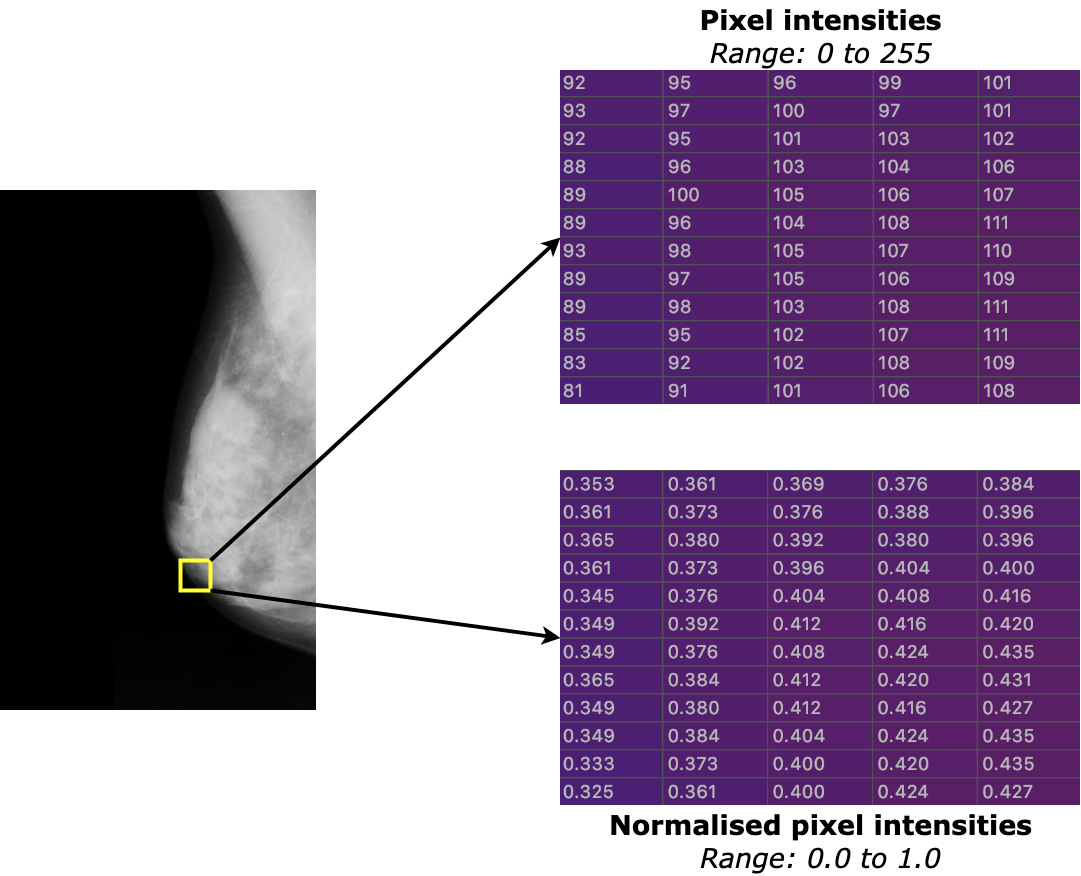
\includegraphics[width=0.9\textwidth]{figures/design/Normalisation example.png}}
\caption{\label{fig:design-Normalisation example}Example of the pixels values that make up a mammogram before and after normalisation.}
\end{figure}

\subsubsection{Label encoding}

As the labels for each mammogram are in categorical string format, they must be encoded into a numerical format. On the one hand, due to the sparse nature of the labels (only three categories), one-hot encoding is chosen for the mini-MIAS dataset, where a single digit may have the value 1 while the others remain at value 0 to tell apart the different labels. The one-hot encodings of the labels can be seen in Table~\ref{tab:one-hot-encoding-example}.

% The data must be fed to the neural network in binary form. One-hot encoding is therefore chosen as it suits the sparse representation of the data, which is made up of only five target categories. Only a single digit may have the value 1 in one-hot encoding, while the others remain at value 0 \cite{lec16}. The one-hot encodings of the target categories can be seen in Figure \ref{fig:one_hot_encoding}.

\begin{table}[h]
\centering
\begin{tabular}{|c|c|}
\hline
\textbf{Categorical format} & \textbf{One-hot encoding} \\ \hline
\textit{Normal}             & 1 0 0            \\ \hline
\textit{Benign}             & 0 1 0            \\ \hline
\textit{Malignant}          & 0 0 1            \\ \hline
\end{tabular}
\caption{Conversion from string (categorical) format to one-hot encoding.}
\label{tab:one-hot-encoding-example}
\end{table}

On the other hand, in the case of binary datasets like CBIS-DDSM, binary encoding can be used instead of one-hot encoding, as seen in Table~\ref{tab:binary-encoding-example}.

\begin{table}[h]
\centering
\begin{tabular}{|c|c|}
\hline
\textbf{Categorical format} & \textbf{Binary encoding} \\ \hline
\textit{Benign}             & 0                        \\ \hline
\textit{Malignant}          & 1                        \\ \hline
\end{tabular}
\caption{Conversion from string (categorical) format to binary encoding.}
\label{tab:binary-encoding-example}
\end{table}

%%%%%%%%%%%%%%%%%%%%

\subsection{Model Training}

At this stage, the training data is ready to be fed into the CNN model. The classification models will learn the processed images from the training set loaded in memory before making their predictions, which will be compared with the ground truth labels for evaluation.

\subsubsection{CNN model}
\label{sec:design-cnn-model-decision}

Due to the small nature of the CBIS-DDSM and mini-MIAS datasets used, state-of-the-art CNN models pre-trained on large general datasets like ImageNet are used rather than creating a CNN from scratch, a technique known as transfer learning (see Section~\ref{sec:litreview-transfer-learning}) that is proven to work on breast cancer detection tasks \citep{Shen2017, Falconi2019}.\\

Different CNN architectures can be used as the base of a custom CNN model tailored for breast cancer detection. This is achieved by using popular CNN architectures available with Keras such as VGG19, ResNet50, InceptionV3, DenseNet121 and MobileNetV2 as the base of the CNN \citep{kerasApplications}. The fully connected layers of these models, which are designed for general classification of natural images into 1,000 different categories \citep{Krizhevsky2012}, are dropped from the model and replaced with a custom MLP. The fully-connected MLP contains hidden layers and an output layer with different activation functions based on the dataset used.\\

If large images are used, then additional convolutional and pooling layers are added before the base model to downsample the image to smaller sizes and learn low-level features, followed by the pre-trained base model, a flatten layer to convert the output from 2D to 1D, and finally the MLP which will make the final prediction. Dropout layers are added in the MLP to avoid overfitting.

\begin{figure}[ht]
\centerline{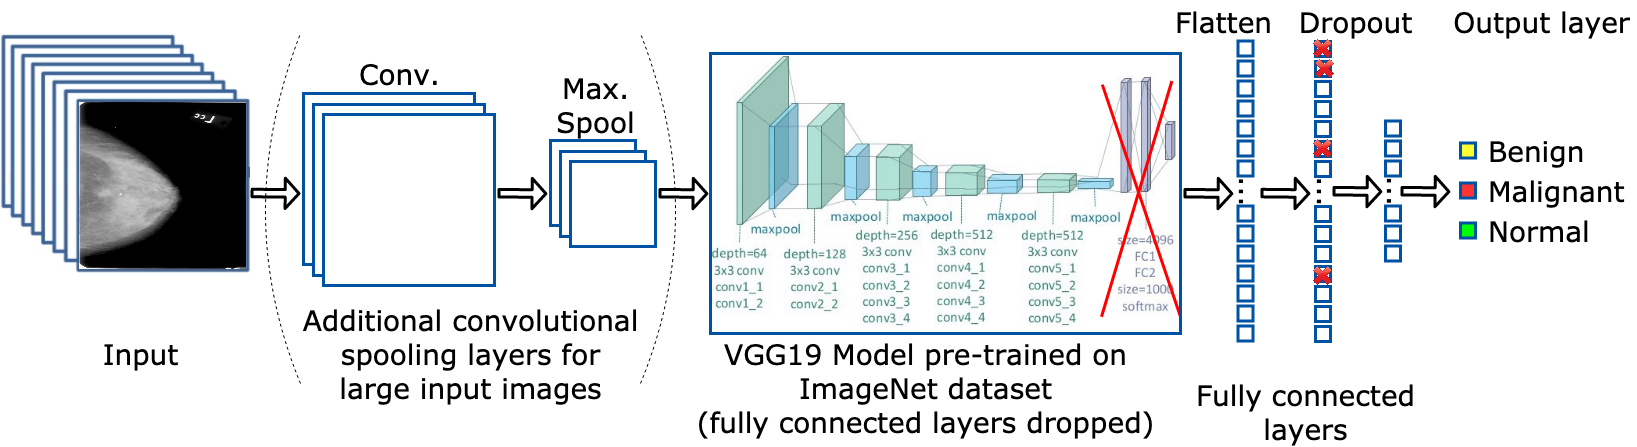
\includegraphics[width=1.2\textwidth]{figures/design/CNN architecture.png}}
\caption{\label{fig:design-CNN architecture}CNN architecture used. VGG19 image retrieved from \url{https://tinyurl.com/rpp49oc}.}
\end{figure}

\subsubsection{Data fitting}

\paragraph{Activation functions}

Different activation functions can be used in the output layer of the CNN (see Figure~\ref{fig:design-activation functions}). Typically, a single neuron with a sigmoid activation function is used for binary problems as it outputs an independent value between 0 and 1 that can be interpreted as a probability of the positive class. Inversely, a softmax activation function transforms the output of the last hidden layer into probabilities for each class that sum up to 1 \citep{Litjens2017}. These probabilities are dependent of each other, as each sample must belong to one class only, making it perfect for multi-class classification of breast mammograms (each sample can only be either normal, benign or malignant, therefore to increase the probability of one class, it must decrease it for another).

\begin{figure}[ht]
\centerline{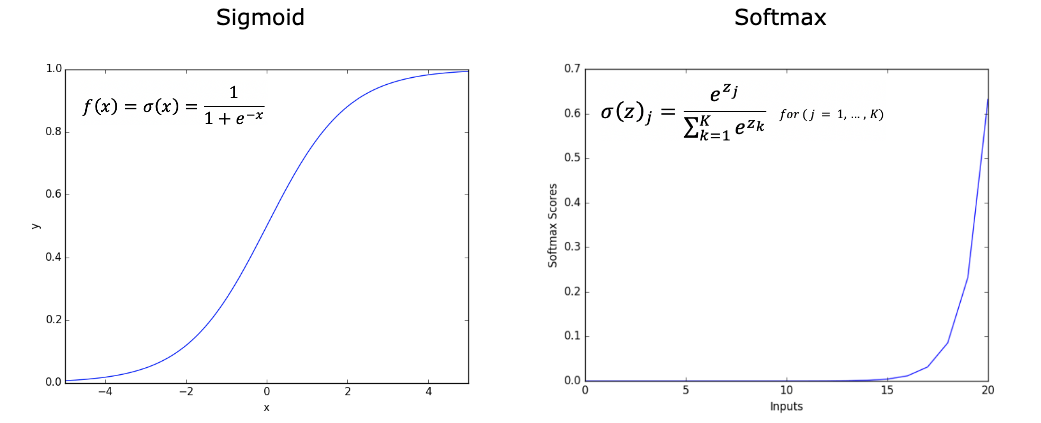
\includegraphics[width=1.1\textwidth]{figures/design/activation functions.png}}
\caption{\label{fig:design-activation functions}Visualisation of the sigmoid and softmax activation functions.}
\end{figure}
% https://glassboxmedicine.com/2019/05/26/classification-sigmoid-vs-softmax/

Resultantly, the output layer will use a sigmoid with the CBIS-DDSM dataset, and a softmax with the mini-MIAS dataset.

\paragraph{Loss function}

Cross entropy is one of the most commonly used loss functions as it can be used for both binary and multi-class tasks \citep{Litjens2017}. Because probabilities are being estimated through the sigmoid and softmax activation functions, cross entropy is the ideal loss function as it heavily penalises the model when a low probability is predicted for the target class \citep{Geron2019}.
% https://www.machinecurve.com/index.php/2019/10/22/how-to-use-binary-categorical-crossentropy-with-keras/
%https://gombru.github.io/2018/05/23/cross_entropy_loss/

\paragraph{Optimiser}

Due to the deep nature of the model, it is important to minimise the number of hyperparameters to control. Adaptive learning rate algorithms usually generalise better than traditional optimisers like Stochastic Gradient Descent (SGD) or momentum, which are slow to converge and require more fine-tuning. The most general adaptive optimiser is \textit{adaptive moment estimation} (Adam), which combines both momentum for more significant steps in the direction of the steepest gradient and Root Mean Square Prop (RMSProp) for accelerating more on steep slopes than small slopes, making it the best choice for this model.
%https://towardsdatascience.com/full-review-on-optimizing-neural-network-training-with-optimizer-9c1acc4dbe78

\paragraph{Transfer learning}
\label{sec:design-transfer-learning-training-phase}

To best make use of the transfer learning technique with the base model's weights instantiated using ImageNet weights, training is separated into two phases:
\begin{enumerate}
    \item All the layers from the base model are frozen, enabling only the custom MLP with fully connected layers to fit the mammogram images. The initial training phase ends once the maximum number of epochs is reached, or the early stopping condition is met.
    \item All the layers are unfrozen, and training is resumed with a smaller learning rate $\alpha = 0.00001$, allowing the base model to slightly alter its weights to adapt to the mammogram dataset while not forgetting the ImageNet knowledge.
\end{enumerate}

\paragraph{Validation set \& early stopping}
\label{sec:design-validation-early-stopping}

To ensure that the model generalises well to unseen  data from the testing set, the training set is further split to form a validation set using a 75\%25\% split on training set; resulting in a 60\%/20\%/20\% of the full dataset. The validation set is used to make predictions at the end of each epoch by calculating the loss and accuracy. These values are then monitored to stop the training before the maximum number of epochs is reached if the validation accuracy or loss do not improve after a certain number of epochs, preventing the model from overfitting the data too much.\\

Due to time constraints, k-fold cross-validation, which divides the training set into $K$ subsets and evaluates the model $K$ times, cannot be used as training the model on the CBIS-DDSM dataset can take anywhere from 1h15m to 8h49 (see Chapter~\ref{ch:chapter-evaluation}), which would be multiplied by a factor of $K$. Therefore, a validation set is used instead.

\paragraph{Fine-tuning}
\label{sec:design-fine-tuning-bagoftricks}

Traditionally, a grid search approach would have been preferred to fine-tune the model's hyperparameters. However, due to the significant training runtime and the number of hyperparameters to fine-tune, a grid search would have been unrealistic given the time frame of the project. Additionally, two attempts at implementing grid search were unsuccessful, as a known bug on the Keras wrapper for Scikit-Learn prevented the use of the \textit{GridSearch class}, and Optuna was incompatible with the current version of Tensorflow I/O being used.\\

Instead, a bag-of-tricks approach is selected, manually trying different deep learning techniques mentioned in this chapter such as using different pre-trained CNN models, amounts of transfer learning, amounts of data augmentation, dropout values and input image sizes.
% over a genetic algorithm to naturally find best hyperparameters.

%%%%%%%%%%%%%%%%%%%%

\subsection{Result Visualisation}
\label{sec:design-results-visualisation}

The following terminology is used to define the metrics used below:
\begin{itemize}
    \item TP: True Positives (positive case correctly predicted as positive);
    \item TN: True Negatives (negative case correctly predicted as negative);
    \item FP: False Positives (negative case incorrectly predicted as positive);
    \item FN: False Negatives (positive case incorrectly predicted as negative).
\end{itemize}

\subsubsection{Overall accuracy}

The imbalanced class distributions (see Section~\ref{sec:design-dataset-balance}) must be taken into account when analysing the classifiers' scores. Indeed, using an evaluation metric such as overall accuracy (see Equation~\ref{eq:accuracy}, \cite{Falconi2019}) would be misleading as it would not be representative of how well the classifier fitted the data. Additionally, in breast cancer detection, detecting FPs and FNs is primordial to avoid interpreting malignant tumours as benign and vice versa, an interpretation which could harm the patient and eventually lead to their death.

\begin{equation}
\label{eq:accuracy}
    Accuracy = \frac{TP + TN}{P + N}
\end{equation}

For instance, if a dumb classifier that always classifies an image as ``normal'' is created, it would achieve 64.28\% accuracy on the mini-MIAS dataset despite  never picking up abnormal cases. Therefore, a mixture of additional metrics should be used to assess how well the model learns the mammograms data and generalises to unseen cases.

\subsubsection{Precision \& recall}

Precision corresponds to the number of correct positive predictions (see Equation~\ref{eq:precision}, \cite{Liu2009}), showing the model's ability to avoid labelling negative instances as positive. 

\begin{equation}
\label{eq:precision}
    Precision = \frac{TP}{TP+FP}
\end{equation}

Recall is the number of positive instances that are correctly predicted (see Equation~\ref{eq:recall}, \cite{Liu2009}), showing how well the model can find all positive instances.

\begin{equation}
\label{eq:recall}
    Recall = \frac{TP}{TP+FN}
\end{equation}

\subsubsection{F1 score}

Together, precision and recall can be combined into a more concise metric, the \textit{F1 score}, which corresponds to the harmonic mean of precision and recall (see Equation \ref{eq:f1-score}, \cite{Geron2019}). To achieve a high F1 score, both precision and recall must be high (unlike a regular mean) because as the precision goes down, the recall goes up, and vice versa, making the F1 score a reliable metric for evaluating a classifier since a balance between precision and recall must be found \citep{Geron2019}.

\begin{equation}
\label{eq:f1-score}
    F_{1} = \frac{2}{\frac{1}{precision} + \frac{1}{recall}} = \frac{TP}{TP+\frac{FN + FP}{2}}
\end{equation}

\subsubsection{Confusion matrix} 

This visual metric plots the number of predictions made for each class for each possible class in a table, with each row corresponding to the actual labels and each column corresponding to a prediction. It is beneficial for detecting which actual classes are being detected the most, and what predicted classes are being misclassified as \citep{Bhardwaj2015, Liu2009}. To further highlight the misclassifications and compare predictions with other classifiers, the confusion matrices are normalised to show a percentage rather than a count.

%%%%%%%%%%%%%%%%%%%%%%%%%%%%%%%%%%%%%%%%%%%%%%%%%%%%%%%%%%%%%%%%%%%%
%%%%%%%%%%%%%%%%%%%%%%%%%%%%%%%%%%%%%%%%%%%%%%%%%%%%%%%%%%%%%%%%%%%%
%%%%%%%%%%%%%%%%%%%%%%%%%%%%%%%%%%%%%%%%%%%%%%%%%%%%%%%%%%%%%%%%%%%%

\section{General Design Decisions}

\subsection{Programming Language}

% Choosing a programming language is one of the most essential aspects to take into account as it is the medium used to transform the system from design to implementation. However, choosing from over 250 different programming languages \citep{tiobe} can be tricky, which is why multiple views have to be evaluated before choosing a programming language. Four popular programming languages are considered for this project: Python, Java, R and  Javascript.\\
% https://becominghuman.ai/best-languages-for-machine-learning-in-2020-6034732dd242

The first element to consider when choosing a programming language is the availability of third-party libraries used for implementing common machine learning functionalities, as well as data pre-processing, manipulation and visualisation techniques found in deep learning systems to avoid manually implementing them. The most commonly used machine learning libraries nowadays are all available in Python \citep{raschka2017python}, including SciKit-Learn \citep{scikit-learn}, Pandas \citep{reback2020pandas}, Matplotlib \citep{Hunter:2007}, NumPy \citep{numpy} and Seaborn \citep{seaborn}. In terms of deep learning libraries, Tensorflow (available in Python, R and Javascript) and PyTorch (available in Python) are  the most popular ones (Appendix~\ref{sec:appendix-keras_vs_pytorch}).\\

In terms of speed, compiled languages are quicker than interpreted languages, but because the main bottleneck in a deep learning system is the training phase of the model, which mainly relies on the library used rather than the language itself, speed is not taken into account. Finally, Python is the favoured language in terms of personal preference, familiarity, and experience, especially when applied to machine learning projects, making it the apparent programming language candidate for this project. For a complete review of the main pros and cons considered between when deciding between Python, Java, R and Javascript, refer to Appendix~\ref{sec:appendix-programming-languages-comparison}.

\subsection{Deep Learning Framework}

Due to the vast nature of the datasets and complexity of the deep learning models to implement, powerful computing resources will be used in the form of Graphical Processing Units (GPU). A GeForce GTX 1060 6GB is provided by the School of Computer Science and remotely accessed via SSH to a lab machine equipped with the GPU in question running on CentOS.\\

To make use of the GPU's computing capabilities, deep learning frameworks with CUDA support (for parallel computing and GPU optimisations), CNN support and pre-trained models should be used. The two most popular deep learning frameworks nowadays are Tensorflow coupled with Keras, and PyTorch. Tensorflow/Keras being relatively older than PyTorch, have got more online support, which is confirmed by the number of daily downloads Keras has compared to PyTorch (ten times more), as well as the number of mentions in academic papers (see figures  in Appendix~\ref{sec:appendix-keras_vs_pytorch}), making them the selected deep learning library.

\subsection{Interface}

A Command-Line Interface (CLI) is selected, allowing arguments and flags to be passed to execute different sections of the code. Arguments control the dataset to use, the CNN model, and the mode to run in (training or testing). Flags control the verbose mode to print more statements in the terminal for debugging purposes. The full set of instructions to run the code can be found in Appendix~\ref{ch:appendix-usage-instructions}.

%%%%%%%%%%%%%%%%%%%%%%%%%%%%%%%%%%%%%%%%%%%%%%%%%%%%%%%%%%%%%%%%%%%%
%%%%%%%%%%%%%%%%%%%%%%%%%%%%%%%%%%%%%%%%%%%%%%%%%%%%%%%%%%%%%%%%%%%%
%%%%%%%%%%%%%%%%%%%%%%%%%%%%%%%%%%%%%%%%%%%%%%%%%%%%%%%%%%%%%%%%%%%%

\section{Design Decisions Summary}

\begin{enumerate}
    \item Datasets:
    \begin{itemize}
        \item CBIS-DDSM (binary classification)
        \item mini-MIAS (multi-class classification)
    \end{itemize}
    
    \item Data pre-processing steps:
    \begin{itemize}
        \item 60/20/20\% train/test/validation splits
        \item Data augmentation
        \item Image normalisation
        \item One-hot encoding (CBIS-DDSM) and binary encoding (mini-MIAS)
    \end{itemize}
    
    \item Model training:
     \begin{enumerate}
        \item Base model: VGG19, ResNet50, InceptionV3, DenseNet121 and MobileNetV2 
        \item Output layer activation function: softmax (CBIS-DDSM) and sigmoid (mini-MIAS)
        \item Optimiser: Adam
        \item Loss function: Cross entropy
        \item Transfer learning
        \item Generalisation to unseen data: validation loss and accuracy early stopping
        \item Fine-tuning: bag-of-tricks approach
    \end{enumerate}
    
    \item Evaluation Metrics:
    \begin{enumerate}
        \item Numerical metrics:
        \begin{itemize}
            \item Overall accuracy
            \item Precision \& recall
            \item F1 score
        \end{itemize}
        \item Visual metrics:
        \begin{itemize}
            \item Confusion matrices (counts)
            \item Normalised confusion matrices
        \end{itemize}
    \end{enumerate}
    
    \item Programming language:
    \begin{enumerate}
        \item Python 3.7
        \item Open-source frameworks:
        \begin{itemize}
            \item Tensorflow \& Keras
            \item Scikit-Learn
            \item NumPy, Pandas, MatplotLib \& Seaborn
        \end{itemize}
    \end{enumerate}
    
    \item Interface: Command-Line Interface
\end{enumerate}
